%=============================================================================%
% PRÉSENTATION PFE - Attijariwafa Bank / ESI
% Optimisation du Réseau d'Agences Bancaires
%=============================================================================%
\documentclass[aspectratio=169, 9pt]{beamer}

%------------------------------------------------------------------------------%
% PACKAGES
%------------------------------------------------------------------------------%
\usepackage[utf8]{inputenc}
\usepackage[T1]{fontenc}
\usepackage[french]{babel}
\usepackage{graphicx}
\usepackage{booktabs}
\usepackage{array}
\usepackage{tikz}
\usepackage{xcolor}
\usepackage{fontawesome5}
\usepackage{multicol}
\usepackage{adjustbox}
\usepackage{ragged2e}
\usepackage{setspace}

\usetikzlibrary{shapes.geometric, arrows.meta, positioning, calc, shadows.blur}

%------------------------------------------------------------------------------%
% COULEURS DU THÈME
%------------------------------------------------------------------------------%
\definecolor{PrimaryDark}{RGB}{255, 255, 255}       % Fond sombre principal
\definecolor{SecondaryDark}{RGB}{248, 250, 252}      % Fond sombre secondaire
\definecolor{AccentOrange}{RGB}{234, 88, 12}      % Orange AWB
\definecolor{AccentBlue}{RGB}{37, 99, 235}        % Bleu accent
\definecolor{AccentGreen}{RGB}{22, 163, 74}       % Vert succès
\definecolor{AccentPurple}{RGB}{124, 58, 237}     % Violet
\definecolor{AccentRed}{RGB}{220, 38, 38}         % Rouge alerte
\definecolor{TextWhite}{RGB}{15, 23, 42}          % Texte clair
\definecolor{TextMuted}{RGB}{100, 116, 139}       % Texte atténué
\definecolor{CardBg}{RGB}{241, 245, 249}          % Fond de carte
\definecolor{Border}{RGB}{203, 213, 225}          % Bordures

%------------------------------------------------------------------------------%
% THÈME BEAMER
%------------------------------------------------------------------------------%
\usetheme{default}
\usecolortheme{default}

% Supprimer barres de navigation
\setbeamertemplate{navigation symbols}{}
\setbeamertemplate{footline}{}

% Fond global
\setbeamercolor{background canvas}{bg=PrimaryDark}
\setbeamercolor{normal text}{fg=TextWhite}

% Titre de frame
\setbeamercolor{frametitle}{fg=TextWhite, bg=}
\setbeamerfont{frametitle}{size=\Large, series=\bfseries}
\setbeamertemplate{frametitle}{%
  \vskip6pt
  \insertframetitle
  \vskip0pt
  {\color{AccentOrange}\rule{\textwidth}{1.2pt}}
  \vskip4pt
}

% Itemize
\setbeamertemplate{itemize item}{\color{AccentOrange}\textbullet}
\setbeamertemplate{itemize subitem}{\color{AccentBlue}\textendash}
\setbeamertemplate{itemize subsubitem}{\color{TextMuted}\textbullet}
\setbeamercolor{itemize item}{fg=AccentOrange}
\setbeamercolor{itemize subitem}{fg=AccentBlue}
\setlength{\leftmargini}{1.2em}
\setlength{\leftmarginii}{1.4em}

% Enumerate
\setbeamertemplate{enumerate item}{\color{AccentOrange}\bfseries\insertenumlabel.}

%------------------------------------------------------------------------------%
% COMMANDES UTILITAIRES
%------------------------------------------------------------------------------%

% Slide de section (intercalaire)
\newcommand{\sectionslide}[2]{%
  \begin{frame}[plain]
    \begin{tikzpicture}[remember picture, overlay]
      \fill[SecondaryDark] (current page.north west) rectangle (current page.south east);
      \fill[AccentOrange] ([yshift=-4.5cm]current page.north west) rectangle ([yshift=-4.55cm]current page.north east);
      \node[anchor=center, text=TextMuted, font=\large] at ([yshift=-3.2cm]current page.center) {#2};
      \node[anchor=center, text=TextWhite, font=\Huge\bfseries] at ([yshift=0.4cm]current page.center) {#1};
    \end{tikzpicture}
  \end{frame}
}

% Carte info avec icône
\newcommand{\infocard}[3]{%
  \begin{tikzpicture}
    \node[fill=CardBg, rounded corners=6pt, minimum width=#1, minimum height=1.6cm, inner sep=8pt, anchor=north west] (box) at (0,0) {};
    \node[anchor=west, text=AccentOrange, font=\Large] at ([xshift=5pt]box.west) {#2};
    \node[anchor=west, text=TextWhite, font=\small] at ([xshift=28pt]box.west) {#3};
  \end{tikzpicture}
}

% Placeholder image
\newcommand{\imgplaceholder}[2]{%
  \begin{tikzpicture}
    \node[fill=CardBg, rounded corners=4pt, minimum width=#1, minimum height=#2, draw=Border, line width=0.5pt] (ph) {};
    \node[text=TextMuted, font=\footnotesize\itshape, text width=0.8*#1, align=center] at (ph.center) {\faImage\ Image à insérer};
  \end{tikzpicture}
}

% Numéro de page personnalisé
\setbeamertemplate{footline}{%
  \begin{tikzpicture}[remember picture,overlay]
    \node[
      anchor=south east,
      text=TextMuted,
      font=\small
    ] at ([xshift=-0.3cm,yshift=0.5cm]current page.south east)
    {\insertframenumber};
  \end{tikzpicture}
}

%=============================================================================%
\begin{document}
%=============================================================================%

%=============================================================================
% SLIDE 1 — PAGE DE GARDE
%=============================================================================
\begin{frame}[plain]
  \begin{tikzpicture}[remember picture, overlay]

    % Logos and Top Center Text
    \node[anchor=north west, inner sep=0pt] at ([xshift=1.2cm, yshift=-0.5cm]current page.north west) {%
      
\includegraphics[height=1.4cm]{logoesi.jpg}%
    };
    
    \node[anchor=north, text=TextWhite, font=\small\bfseries, align=center] at ([yshift=-0.6cm]current page.north) {%
      Royaume du Maroc\\[2pt]
      Haut-Commissariat au Plan
    };

    \node[anchor=north east, inner sep=0pt] at ([xshift=-1.2cm, yshift=-0.5cm]current page.north east) {%
      
\includegraphics[height=1.4cm]{logoawb.png}%
    };


    % Lignes et Titre
    \draw[AccentOrange, line width=1.8pt] ([xshift=1.5cm, yshift=1.0cm]current page.west) -- ([xshift=-1.5cm, yshift=1.0cm]current page.east);
    
    \node[anchor=center, text=TextWhite, font=\Large\bfseries, align=center, text width=13cm] at ([yshift=0cm]current page.center) {%
      Development d'une Plateforme d'Intelligence Territoriale pour\\[4pt]
      l'Optimisation du Réseau d'Agences Bancaires%
    };

    \draw[AccentOrange, line width=1.8pt] ([xshift=1.5cm, yshift=-1.0cm]current page.west) -- ([xshift=-1.5cm, yshift=-1.0cm]current page.east);

    % Soutenu par
    \node[anchor=north, text=TextWhite, font=\normalsize, align=center] at ([yshift=-1.5cm]current page.center) {%
      Soutenu par : \textbf{Salah Eddine AHADAF}\\[4pt]
      Juin 2026
    };

    % Jury
    \node[anchor=south west, text=TextWhite, font=\small, align=left] at ([xshift=1.2cm, yshift=1.2cm]current page.south west) {%
      \textbf{Membres du jury :}\\[4pt]
      $\bullet$ Président(e) : Pr \\[2pt]
      $\bullet$ Encadrante : Pr Basma BOUKENZE\\[2pt]
      $\bullet$ Tuteur : M. Ahmed EL RHEDDANE
    };

    % Année universitaire
    \node[anchor=south east, text=TextWhite, font=\small] at ([xshift=-1.2cm, yshift=1.2cm]current page.south east) {%
      Année universitaire : 2025/2026
    };

  \end{tikzpicture}
\end{frame}

%=============================================================================
% SLIDE 2 — PLAN DE LA PRÉSENTATION
%=============================================================================
%=============================================================================
% SLIDE 2 — PLAN DE LA PRÉSENTATION
%=============================================================================
\begin{frame}{Plan de la Présentation}
  \begin{columns}[T]
    \begin{column}{0.7\textwidth} 
      % La commande \Large augmente la taille de la police
      \Large 
      \begin{enumerate}
        \item[\color{AccentOrange}\textbf{1}] \textbf{Introduction}
        
        \vspace{0.8cm} 
        \item[\color{AccentOrange}\textbf{2}] \textbf{Implémentation}
        
        \vspace{0.8cm}
        \item[\color{AccentOrange}\textbf{3}] \textbf{Démonstration de la solution}
        
        \vspace{0.8cm}
        \item[\color{AccentOrange}\textbf{4}] \textbf{Conclusion et perspectives}
      \end{enumerate}
    \end{column}
    
    \begin{column}{0.25\textwidth}
      % Cette colonne de droite reste vide, ce qui force le texte à rester à gauche
    \end{column}
  \end{columns}
\end{frame}

%=============================================================================
% SECTION 1 — CONTEXTE
%=============================================================================
\sectionslide{Introduction : Contexte et Organisme d'Accueil}{Partie 1}

%=============================================================================
% SLIDE 3 — ATTIJARIWAFA BANK
%=============================================================================
\begin{frame}{Attijariwafa Bank --- Premier Groupe Bancaire du Maghreb}
  \begin{columns}[T]
    \begin{column}{0.55\textwidth}
      \begin{itemize}
        \item Fondé en 2003 (fusion BCM \& Wafabank)
        \item \textbf{Premier groupe bancaire} au Maghreb et en Afrique de l'Ouest
        \item Présent dans \textbf{25 pays} à travers le monde
        \item \textbf{+20 000 collaborateurs}
        \item Total bilan : \textbf{+750 milliards MAD} (2024)
        \item PNB consolidé : \textbf{32,2 milliards MAD}
      \end{itemize}
      \vspace{0.3cm}
      {\color{AccentOrange}\faMapMarkerAlt} \textbf{+6 600 agences} à travers le réseau international, dont \textbf{+3 800 au Maroc}.
    \end{column}
    \begin{column}{0.42\textwidth}
      % PLACEHOLDER: insérer filiale-mondiale.png ou autre image AWB
      \begin{center}
        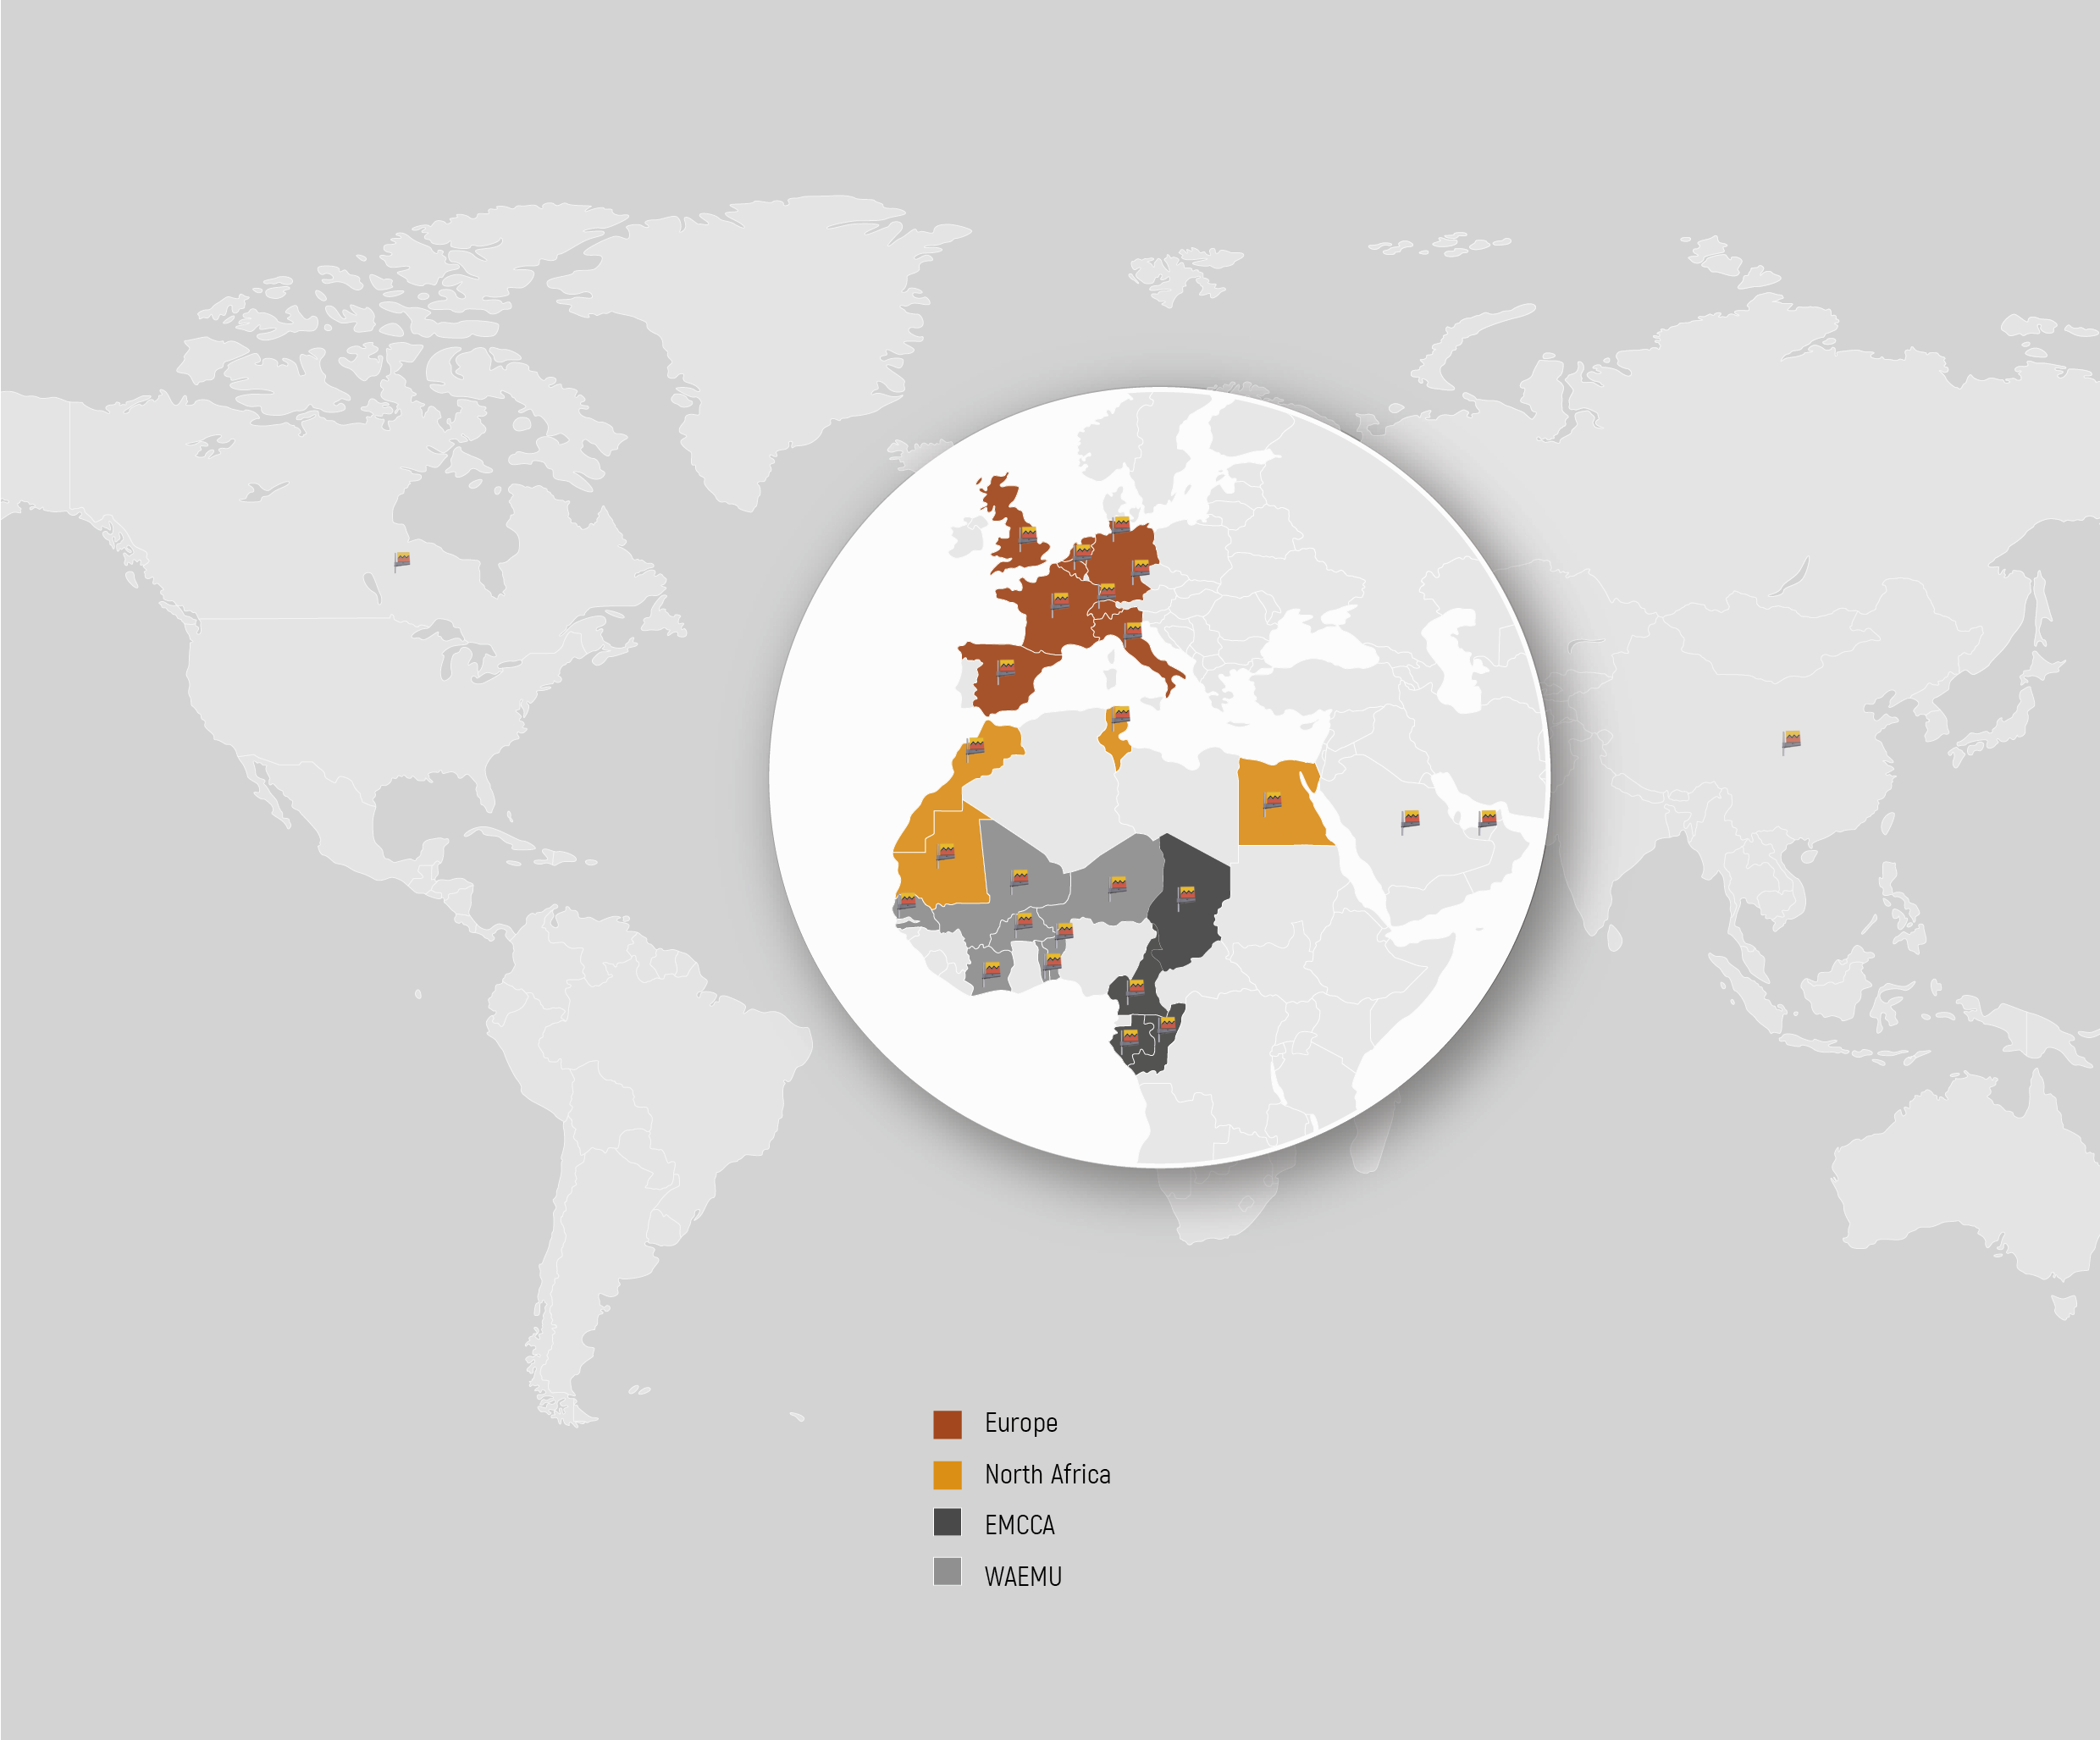
\includegraphics[width=\textwidth]{filiale-mondiale.png}
      \end{center}
    \end{column}
  \end{columns}
\end{frame}

%=============================================================================
% SLIDE 4 — CONTEXTE DU PROJET
%=============================================================================
\begin{frame}{Contexte du Projet}
  \vspace{0.2cm}
  Le secteur bancaire marocain traverse une \textbf{transformation majeure}. La digitalisation des services, l'évolution des habitudes des clients et l'intensification de la concurrence imposent une \textbf{révision stratégique de la présence physique}.

  \vspace{0.4cm}
  \begin{columns}[T]
    \begin{column}{0.48\textwidth}
      {\color{AccentRed}\faExclamationTriangle} \textbf{Constats : Les aspects}
      \begin{itemize}
        \item Agences trop proches qui se cannibalisent
        \item Zones à fort potentiel non couvertes
        \item Décisions d'implantation basées sur l'intuition
        \item Absence d'outil d'évaluation objective
      \end{itemize}
    \end{column}
    \begin{column}{0.48\textwidth}
      {\color{AccentGreen}\faLightbulb} \textbf{Opportunité}
      \begin{itemize}
        \item Exploiter la donnée géospatiale (POI)
        \item Appliquer le Machine Learning au scoring territorial
        \item Automatiser l'évaluation du réseau
        \item Fournir un outil d'aide à la bonne décision visuel et interactif
      \end{itemize}
    \end{column}
  \end{columns}
\end{frame}

%=============================================================================
% SECTION 2 — PROBLÉMATIQUE ET OBJECTIFS
%=============================================================================
\sectionslide{Introduction : Problématique et Objectifs}{Partie 1}

%=============================================================================
% SLIDE 5 — PROBLÉMATIQUE
%=============================================================================
\begin{frame}{Problématique}
  \vspace{0.4cm}
  \begin{center}
    \begin{tikzpicture}
      \node[fill=CardBg, rounded corners=8pt, inner sep=14pt, text width=13cm, align=center, draw=AccentOrange, line width=1pt] {
        {\color{TextWhite}\large\itshape
          «\,Comment aider Attijariwafa Bank à analyser et optimiser son réseau d'agences à partir de la donnée géospatiale et des points d'intérêt, afin d'améliorer la prise de décision stratégique tout en maintenant une couverture territoriale cohérente sur l'ensemble du Maroc\,?»
        }
      };
    \end{tikzpicture}
  \end{center}

  \vspace{0.4cm}
  Cette question se décline en \textbf{trois axes} :
  \begin{enumerate}
    \item \textbf{Évaluer} objectivement chaque agence selon son environnement territorial
    \item \textbf{Optimiser} le réseau existant (fusions, fermetures, investissements ciblés)
    \item \textbf{Recommander} de nouveaux emplacements à fort potentiel
  \end{enumerate}
\end{frame}

%=============================================================================
% SLIDE 6 — OBJECTIFS
%=============================================================================
%=============================================================================
% SLIDE 6 — OBJECTIFS
%=============================================================================
\begin{frame}{Objectifs du Projet}
  \vspace{0.2cm}
  \begin{columns}[T]
    \begin{column}{0.55\textwidth}
      {\color{AccentOrange}\faBullseye} \textbf{Objectif principal}

      \vspace{0.2cm}
      Concevoir une \textbf{plateforme d'Intelligence Territoriale} capable de transformer des données géospatiales brutes en recommandations stratégiques actionnables.

      \vspace{0.4cm}
      \textbf{À travers :}
      \begin{enumerate}
        \item La collecte et centraliser les données POI depuis 3 sources
        \item Calcule des 7 scores normalisés par agence
        \item segmentation du réseau via clustering K-Means
        \item Détection des zones de cannibalisation
        \item Sélection des meilleurs emplacements candidats
        \item Catégorisation des agences sur une matrice stratégique BCG
      \end{enumerate}
    \end{column}
    \begin{column}{0.40\textwidth}
      {\color{AccentBlue}\faCogs} \textbf{Modules générateurs}
      
      \vspace{0.2cm}
      \begin{itemize}
        \item Tableau de bord interactif multi-modules
        \item Pipeline de scoring automatisé
        \item Moteur de sélection de sites
        \item Module d'optimisation réseau
      \end{itemize}
    \end{column}
  \end{columns}
\end{frame}


%=============================================================================
% SECTION 4 — CONCEPTION FONCTIONNELLE
%=============================================================================
\sectionslide{Implementation : Conception Fonctionnelle}{Partie 2}

%=============================================================================
% SLIDE 8 — EXIGENCES FONCTIONNELLES
%=============================================================================
%=============================================================================
% SLIDE 8 — EXIGENCES FONCTIONNELLES
%=============================================================================
\begin{frame}{Exigences Fonctionnelles}
  \vspace{0.1cm}
  {\footnotesize
  
  {\color{AccentBlue}\faSearch} \textbf{Axe 1 : ÉVALUER le réseau existant}
  
  \vspace{0.1cm}
  \begin{tabular}{@{}>{\color{AccentOrange}\bfseries}p{3.5cm} p{10.5cm}@{}}
    \cmidrule(l{0cm}r{0.2cm}){1-2}
    \color{TextWhite}\textbf{Module} & \color{TextWhite}\textbf{Fonctionnalités clés} \\
    \cmidrule(l{0cm}r{0.2cm}){1-2}
    Enrichissement & Scraping intégré multi-sources, nettoyage automatisé, boucle d'auto-alimentation \\[2pt]
    Analyse du réseau & Calculer 7 scores normalisés, segmenter par clustering, identifier la cannibalisation \\
    \cmidrule(l{0cm}r{0.2cm}){1-2}
  \end{tabular}

  \vspace{0.3cm}
  {\color{AccentGreen}\faChartLine} \textbf{Axe 2 : OPTIMISER les performances}
  
  \vspace{0.1cm}
  \begin{tabular}{@{}>{\color{AccentOrange}\bfseries}p{3.5cm} p{10.5cm}@{}}
    \cmidrule(l{0cm}r{0.2cm}){1-2}
    \color{TextWhite}\textbf{Module} & \color{TextWhite}\textbf{Fonctionnalités clés} \\
    \cmidrule(l{0cm}r{0.2cm}){1-2}
    Optimisation réseau & Modèle prédictif XGBoost, calculer ratio de performance, catégoriser sur matrice BCG \\
    \cmidrule(l{0cm}r{0.2cm}){1-2}
  \end{tabular}

  \vspace{0.3cm}
  {\color{AccentPurple}\faMapMarkerAlt} \textbf{Axe 3 : RECOMMANDER de nouveaux sites}
  
  \vspace{0.1cm}
  \begin{tabular}{@{}>{\color{AccentOrange}\bfseries}p{3.5cm} p{10.5cm}@{}}
    \cmidrule(l{0cm}r{0.2cm}){1-2}
    \color{TextWhite}\textbf{Module} & \color{TextWhite}\textbf{Fonctionnalités clés} \\
    \cmidrule(l{0cm}r{0.2cm}){1-2}
    Sélection de sites & Générer grille de candidats, filtrer spatialement, prédire le revenu, classer par score \\[2pt]
    Restitution & Dashboard interactif, cartes, graphiques, export CSV/JSON \\
    \cmidrule(l{0cm}r{0.2cm}){1-2}
  \end{tabular}
  }
\end{frame}

%=============================================================================
% SLIDE 9 — WORKFLOW DU PROJET
%=============================================================================
\begin{frame}{Workflow Global de la Plateforme}
  \begin{center}
    % PLACEHOLDER: insérer workflow_diagram.png (Généré depuis Mermaid)
    \includegraphics[height=0.82\textheight]{workflow_diagram.png}
  \end{center}
\end{frame}

%=============================================================================
% SECTION 5 — CONCEPTION TECHNIQUE
%=============================================================================
\sectionslide{Implementation : Conception Technique}{Partie 2}

%=============================================================================
% SLIDE 11 — ARCHITECTURE DE DONNÉES
%=============================================================================
\begin{frame}{Pipeline de Données et Ingénierie des Caractéristiques}
  \vspace{0.1cm}
  \begin{columns}[T]
    \begin{column}{0.48\textwidth}
      {\color{AccentOrange}\faDatabase} \textbf{Sources de données}
      \begin{itemize}
        \item \textbf{OpenStreetMap} --- POI libres
        \item \textbf{Overture Maps Foundation} --- Données Microsoft/Meta
        \item \textbf{Google Maps} --- Scraping enrichi
        \item \textbf{Données internes AWB} --- Revenus, positions
      \end{itemize}
      \vspace{0.3cm}
      {\color{AccentBlue}\faBroom} \textbf{Nettoyage}
      \begin{itemize}
        \item Classification en 6 catégories de POI
        \item Dédoublonnage géométrique strict (lat/lng)
        \item Validation des coordonnées GPS
      \end{itemize}
    \end{column}
    \begin{column}{0.48\textwidth}
      {\color{AccentGreen}\faChartLine} \textbf{7 Scores normalisés (0--1)}

      \vspace{0.15cm}
      \renewcommand{\arraystretch}{1.1}
      {\footnotesize
      \begin{tabular}{@{}l l@{}}
        \color{AccentOrange}$S_1$ & Score Commercial \\
        \color{AccentOrange}$S_2$ & Score Bureau \\
        \color{AccentOrange}$S_3$ & Score Résidentiel \\
        \color{AccentOrange}$S_4$ & Score Accessibilité \\
        \color{AccentOrange}$S_5$ & Score Concurrence {\color{AccentRed}(pénalisant)} \\
        \color{AccentOrange}$S_6$ & Score Cannibalisation {\color{AccentRed}(pénalisant)} \\
        \color{AccentOrange}$S_7$ & Densité de Population \\
      \end{tabular}
      }

      \vspace{0.3cm}
      {\color{AccentPurple}\faCalculator} \textbf{Score Composite}

      \vspace{0.1cm}
      {\small $C = \alpha S_1 + \beta S_2 + \gamma S_3 + \delta S_4 - \epsilon S_5 - \zeta S_6$}
    \end{column}
  \end{columns}
\end{frame}

%=============================================================================
% SLIDE 12 — STACK TECHNIQUE
%=============================================================================
\begin{frame}{Outils et technologies}
  \vspace{0.1cm}
  \begin{center}
  {\small
  \begin{tabular}{@{}>{\bfseries\color{AccentOrange}}l p{5cm} p{5.5cm}@{}}
    \toprule
    \color{TextWhite}\textbf{Couche} & \color{TextWhite}\textbf{Technologie} & \color{TextWhite}\textbf{Rôle} \\
    \midrule
    Frontend & Streamlit & Tableau de bord interactif \\[3pt]
    Cartographie & Folium + Leaflet.js & Cartes interactives \\[3pt]
    Visualisation & Plotly & Graphiques analytiques \\[3pt]
    ML / Scoring & Scikit-learn, XGBoost & Modèles prédictifs \\[3pt]
    Analyse spatiale & SciPy (cKDTree) & Recherche de proximité \\[3pt]
    Données & Pandas, NumPy & Manipulation tabulaire \\[3pt]
    Collecte POI & Google Maps Scraper & Enrichissement des données \\[3pt]
    Langage & Python 3 & Langage principal \\
    \bottomrule
  \end{tabular}
  }
  \end{center}
\end{frame}
\sectionslide{Implementation : Les principaux Scénario}{Partie 2}
%=============================================================================
% SECTION 6 — UC1 ÉVALUATION RÉSEAU
%=============================================================================
\sectionslide{SC1 --- Évaluation du Réseau Existant}{Partie 2}

%=============================================================================
% SLIDE 13 — DISTRIBUTION ET CLUSTERING
%=============================================================================
\begin{frame}{Analyse Exploratoire et Segmentation K-Means}
  \begin{columns}[T]
    \begin{column}{0.48\textwidth}
      {\color{AccentOrange}\faChartBar} \textbf{Distribution du Score Composite}

      \vspace{0.2cm}
      % PLACEHOLDER: insérer figures/composite_dist.png
      \includegraphics[width=\textwidth]{composite_dist.png}

      \vspace{0.1cm}
      {\footnotesize Moyenne = 0.490, Médiane = 0.576. Réseau polarisé entre zones denses et zones rurales.}
    \end{column}
    \begin{column}{0.48\textwidth}
      {\color{AccentBlue}\faProjectDiagram} \textbf{Projection PCA des 5 Clusters}

      \vspace{0.2cm}
      % PLACEHOLDER: insérer figures/pca_clusters.png
      \includegraphics[width=\textwidth]{pca_clusters.png}

      \vspace{0.1cm}
      {\footnotesize PC1 (72.5\%) sépare zones denses/rurales. PC2 (10.1\%) discrimine profils commerciaux/résidentiels.}
    \end{column}
  \end{columns}
\end{frame}

%=============================================================================
% SLIDE 14 — PROFILS DES CLUSTERS
%=============================================================================
\begin{frame}{Les 5 Profils d'Agences Identifiés}
  \vspace{0.1cm}
  \begin{columns}[T]
    \begin{column}{0.45\textwidth}
      {\small
      \renewcommand{\arraystretch}{1.2}
      \begin{tabular}{@{}l c r@{}}
        \toprule
        \color{TextWhite}\textbf{Cluster} & \color{TextWhite}\textbf{N} & \color{TextWhite}\textbf{\%} \\
        \midrule
        {\color{AccentGreen}High Performer} & 396 & 33.1\% \\
        {\color{AccentBlue}Commercial Hub} & 294 & 24.5\% \\
        {\color{AccentPurple}Residential Anchor} & 181 & 15.1\% \\
        {\color{AccentOrange}At Risk} & 208 & 17.4\% \\
        {\color{AccentRed}Underperformer} & 119 & 9.9\% \\
        \midrule
        \textbf{Total} & \textbf{1\,198} & \textbf{100\%} \\
        \bottomrule
      \end{tabular}
      }
    \end{column}
    \begin{column}{0.52\textwidth}
      % PLACEHOLDER: insérer figures/radar_charts.png
      \includegraphics[width=\textwidth]{radar_charts.png}
    \end{column}
  \end{columns}
\end{frame}

%=============================================================================
% SLIDE 15 — BENCHMARKING RÉGRESSION
%=============================================================================
\begin{frame}{Benchmarking --- Modèles de Régression}
  \vspace{0.1cm}
  \begin{columns}[T]
    \begin{column}{0.42\textwidth}
      {\small
      \renewcommand{\arraystretch}{1.15}
      \begin{tabular}{@{}l c c@{}}
        \toprule
        \color{TextWhite}\textbf{Modèle} & \color{TextWhite}\textbf{$R^2$ CV} & \color{TextWhite}\textbf{RMSE} \\
        \midrule
        OLS / Ridge & 0.866 & 1.02M \\
        Gradient Boosting & 0.871 & 1.01M \\
        XGBoost & 0.863 & 1.04M \\
        \textbf{Random Forest} & \textbf{0.884} & \textbf{0.95M} \\
        \bottomrule
      \end{tabular}
      }

      \vspace{0.3cm}
      Le \textbf{Random Forest} atteint le meilleur $R^2 = 0.884$ en validation croisée à 5 plis, confirmant sa capacité à capturer les relations non-linéaires entre les scores spatiaux et le revenu.
    \end{column}
    \begin{column}{0.55\textwidth}
      % PLACEHOLDER: insérer figures/regression_benchmark.png
      \includegraphics[width=\textwidth]{regression_benchmark.png}
    \end{column}
  \end{columns}
\end{frame}

%=============================================================================
% SLIDE 16 — FEATURE IMPORTANCE
%=============================================================================
\begin{frame}{Importance des Caractéristiques Spatiales}
  \begin{columns}[T]
    \begin{column}{0.55\textwidth}
      \vspace{0.3cm}
      % PLACEHOLDER: insérer figures/xgboost_importance.png
      \includegraphics[width=\textwidth]{xgboost_importance.png}
    \end{column}
    \begin{column}{0.42\textwidth}
      \vspace{0.3cm}
      L'analyse par gain moyen (XGBoost) révèle la hiérarchie des facteurs territoriaux :

      \vspace{0.3cm}
      \begin{enumerate}
        \item {\color{AccentOrange}\textbf{Score Commercial}} --- Prédicteur dominant
        \item {\color{AccentBlue}Densité de Population}
        \item {\color{AccentGreen}Score Bureau}
        \item {\color{AccentPurple}Score Résidentiel}
        \item Score Accessibilité
        \item Score Concurrence
      \end{enumerate}

      \vspace{0.3cm}
      {\footnotesize\color{TextMuted} L'environnement commercial immédiat est le facteur le plus déterminant du revenu d'une agence bancaire.}
    \end{column}
  \end{columns}
\end{frame}

%=============================================================================
% SLIDE 17 — CLASSIFICATION STRATÉGIQUE
%=============================================================================
\begin{frame}{Benchmarking --- Classification Stratégique}
  \vspace{0.1cm}
  \begin{columns}[T]
    \begin{column}{0.42\textwidth}
      Chaque agence est classée en 3 catégories d'action selon son revenu :
      \begin{itemize}
        \item {\color{AccentGreen}\textbf{KEEP}} --- Revenu > 11M MAD
        \item {\color{AccentOrange}\textbf{REVIEW}} --- 6M--11M MAD
        \item {\color{AccentRed}\textbf{CLOSE}} --- Revenu < 6M MAD
      \end{itemize}

      \vspace{0.3cm}
      {\small
      \begin{tabular}{@{}l c@{}}
        \toprule
        \color{TextWhite}\textbf{Modèle} & \color{TextWhite}\textbf{Accuracy} \\
        \midrule
        \textbf{Rég. Logistique} & \textbf{82.9\%} \\
        XGBoost & 82.1\% \\
        Random Forest & 81.7\% \\
        KNN & 81.3\% \\
        \bottomrule
      \end{tabular}
      }
    \end{column}
    \begin{column}{0.55\textwidth}
      % PLACEHOLDER: insérer figures/classification_benchmark.png
      \includegraphics[width=\textwidth]{classification_benchmark.png}
    \end{column}
  \end{columns}
\end{frame}

%=============================================================================
% SECTION 7 — UC2 SÉLECTION DE SITES
%=============================================================================
\sectionslide{SC2 --- Sélection de Nouveaux Sites}{Partie 2}

%=============================================================================
% SLIDE 18 — PIPELINE DE SÉLECTION
%=============================================================================
\begin{frame}{Pipeline de Sélection de Nouveaux Sites}
  \vspace{0.2cm}
  \begin{center}
  \begin{tikzpicture}[node distance=0.4cm and 0.6cm,
    block/.style={fill=CardBg, rounded corners=4pt, draw=Border, line width=0.5pt,
                  minimum height=1cm, minimum width=3cm, text=TextWhite, font=\footnotesize,
                  align=center, text width=2.8cm},
    arrow/.style={-{Stealth[length=5pt]}, color=AccentOrange, line width=1pt}]

    \node[block] (grid) {Génération de la\\grille territoriale};
    \node[block, right=of grid] (filter) {Filtrage spatial\\(côte, proximité)};
    \node[block, right=of filter] (score) {Scoring POI\\inverse-distance};
    \node[block, right=of score] (density) {Densité de\\population};
    \node[block, below=0.6cm of grid] (ref) {Sélection agences\\de référence (Top 10\%)};
    \node[block, right=of ref] (sim) {Similarité cosinus\\candidats vs benchmark};
    \node[block, right=of sim] (predict) {Prédiction revenu\\(Random Forest)};
    \node[block, right=of predict] (top) {Score combiné\\et Top 20};

    \draw[arrow] (grid) -- (filter);
    \draw[arrow] (filter) -- (score);
    \draw[arrow] (score) -- (density);
    \draw[arrow] (density) -- ++(0,-0.8) -| (ref);
    \draw[arrow] (ref) -- (sim);
    \draw[arrow] (sim) -- (predict);
    \draw[arrow] (predict) -- (top);
  \end{tikzpicture}
  \end{center}

  \vspace{0.3cm}
  {\small
  \textbf{Score Combiné} = $W_{POI} \times S_{POI} + W_{SIM} \times S_{similarité} + W_{POP} \times S_{population}$

  \vspace{0.2cm}
  \textbf{Contraintes de diversité} : max 2 sites par ville, distance minimale de 700m entre les candidats retenus.
  }
\end{frame}

%=============================================================================
% SLIDE 19 — RÉSULTATS SITE SELECTION
%=============================================================================
\begin{frame}{Résultats --- Sélection de Nouveaux Sites}
  \begin{center}
    % PLACEHOLDER: insérer screenshot_runsite_results.png
    \includegraphics[width=0.88\textwidth]{screenshot_runsite_results.png}
  \end{center}

  \vspace{0.1cm}
  {\footnotesize Carte interactive affichant les 20 sites recommandés (étoiles orange) superposés aux agences existantes. Chaque candidat est accompagné de son revenu prédit et de son score de similarité aux meilleures agences du réseau.}
\end{frame}

%=============================================================================
% SECTION 8 — UC3 OPTIMISATION RÉSEAU (BCG)
%=============================================================================
\sectionslide{SC3 --- Optimisation du Réseau}{Partie 2}

%=============================================================================
% SLIDE 20 — GAP ANALYSIS CONCEPT
%=============================================================================
\begin{frame}{Gap Analysis --- Isoler Potentiel vs Exécution}
  \vspace{0.2cm}
  L'idée fondamentale est de séparer \textbf{ce que l'emplacement devrait rapporter} (potentiel géographique) de \textbf{ce que l'agence rapporte réellement} (exécution managériale).

  \vspace{0.4cm}
  \begin{columns}[T]
    \begin{column}{0.48\textwidth}
      {\color{AccentOrange}\faCogs} \textbf{Méthode}
      \begin{enumerate}
        \item Entraîner un XGBoost sur les scores spatiaux $\rightarrow$ prédire le revenu attendu $\hat{Y}_i$
        \item Calculer le ratio de performance : $$\text{Ratio}_i = \frac{Y_i^{réel}}{\hat{Y}_i^{prédit}}$$
        \item $\text{Ratio} > 1$ : sur-performance managériale
        \item $\text{Ratio} < 1$ : sous-performance / destruction de valeur
      \end{enumerate}
    \end{column}
    \begin{column}{0.48\textwidth}
      {\color{AccentBlue}\faThLarge} \textbf{Matrice Stratégique BCG}
      \vspace{0.2cm}

      {\small
      \begin{tabular}{@{}l p{5.8cm}@{}}
        {\color{AccentGreen}\textbf{FLAGSHIP}} & Fort potentiel + sur-performance \\[3pt]
        {\color{AccentOrange}\textbf{REVIEW}} & Fort potentiel + sous-performance \\[3pt]
        {\color{AccentBlue}\textbf{MONITOR}} & Faible potentiel + sur-performance \\[3pt]
        {\color{AccentRed}\textbf{CLOSE}} & Faible potentiel + sous-performance \\[3pt]
        {\color{AccentPurple}\textbf{MERGE}} & CLOSE/REVIEW avec un FLAGSHIP à $<$\,1.2\,km \\
      \end{tabular}
      }
    \end{column}
  \end{columns}
\end{frame}

%=============================================================================
% SLIDE 21 — MATRICE BCG
%=============================================================================
\begin{frame}{Matrice BCG Spatiale --- Résultats}
  \begin{center}
    % PLACEHOLDER: insérer figures/bcg_matrix.png
    \includegraphics[width=0.75\textwidth]{bcg_matrix.png}
  \end{center}

  \vspace{0.1cm}
  {\footnotesize Chaque point représente une agence. L'axe X montre le potentiel prédit (XGBoost), l'axe Y le revenu réel. La diagonale $y=x$ représente la ligne d'espérance de potentiel.}
\end{frame}

%=============================================================================
% SLIDE 22 — RÉSULTATS BCG
%=============================================================================
\begin{frame}{Répartition Stratégique des 1\,196 Agences}
  \vspace{0.2cm}
  \begin{columns}[T]
    \begin{column}{0.45\textwidth}
      {\small
      \renewcommand{\arraystretch}{1.3}
      \begin{tabular}{@{}l c r@{}}
        \toprule
        \color{TextWhite}\textbf{Catégorie} & \color{TextWhite}\textbf{N} & \color{TextWhite}\textbf{\%} \\
        \midrule
        {\color{AccentGreen}\textbf{FLAGSHIP}} & 514 & 42.9\% \\
        {\color{AccentOrange}\textbf{REVIEW / INVEST}} & 86 & 7.2\% \\
        {\color{AccentBlue}\textbf{MONITOR}} & 85 & 7.1\% \\
        {\color{AccentRed}\textbf{CLOSE}} & 513 & 42.8\% \\
        \bottomrule
      \end{tabular}
      }
    \end{column}
    \begin{column}{0.52\textwidth}
      {\color{AccentOrange}\faExclamationCircle} \textbf{Résultats clés}

      \vspace{0.2cm}
      \begin{itemize}
        \item \textbf{86 agences} à fort potentiel sous-exploité identifiées --- opportunité d'investissement ciblé
        \item \textbf{513 agences} en zone à faible potentiel avec sous-performance --- candidates à la rationalisation
        \item Détection automatique des fusions spatiales (cKDTree, rayon 1.2\,km)
      \end{itemize}

      \vspace{0.2cm}
      {\footnotesize\color{TextMuted} Les seuils (sur-performance > 1.15, sous-performance < 0.85) sont configurables par l'utilisateur.}
    \end{column}
  \end{columns}
\end{frame}

%=============================================================================
% SLIDE 23 — FUSIONS GÉOSPATIALES
%=============================================================================
\begin{frame}{Fusions Géospatiales Intelligentes}
  \begin{columns}[T]
    \begin{column}{0.55\textwidth}
      \vspace{0.2cm}
      % PLACEHOLDER: insérer screenshot_bcg_scatter.png
      \includegraphics[width=\textwidth]{screenshot_bcg_scatter.png}
    \end{column}
    \begin{column}{0.42\textwidth}
      \vspace{0.2cm}
      Pour chaque agence marquée \textbf{CLOSE} ou \textbf{REVIEW}, le système vérifie s'il existe un \textbf{FLAGSHIP} à proximité (\textless\,1.2\,km).

      \vspace{0.3cm}
      Si une agence d'excellence est proche, la recommandation est convertie en \textbf{\color{AccentPurple}MERGE} --- fusion stratégique qui :
      \begin{itemize}
        \item Réduit les coûts opérationnels
        \item Préserve la couverture géographique
        \item Concentre les ressources sur l'agence performante
      \end{itemize}
    \end{column}
  \end{columns}
\end{frame}

%=============================================================================
% SECTION 9 — DÉMONSTRATION DASHBOARD
%=============================================================================
\sectionslide{Démonstration de la solution}{Partie 3}

%=============================================================================
% SLIDE 24 — ARCHITECTURE DASHBOARD
%=============================================================================
\begin{frame}{Architecture du Platforme --- 10 Modules}
  \vspace{0.1cm}
  {\footnotesize
  \renewcommand{\arraystretch}{1.1}
  \begin{tabular}{@{}>{\color{AccentOrange}\bfseries}c l p{7.5cm}@{}}
    \toprule
    \color{TextWhite}\textbf{\#} & \color{TextWhite}\textbf{Module} & \color{TextWhite}\textbf{Description} \\
    \midrule
    1 & Map & Vue cartographique du réseau national \\
    2 & Rankings & Classement des agences par score composite \\
    3 & ML Clusters & Projection PCA et profils d'agences \\
    4 & Mergers & Détection de cannibalisation inter-agences \\
    5 & Cities & Analyse comparative par ville \\
    6 & Deep Dive & Fiche d'audit individuelle par agence \\
    7 & Scoring Table & Tableau brut des scores de toutes les agences \\
    8 & Run Site Selection & Moteur de découverte interactif \\
    9 & Network Optimization & Matrice BCG et restructuration spatiale \\
    10 & Data Enrichment & Scraping Google Maps et pipeline de nettoyage \\
    \bottomrule
  \end{tabular}
  }
\end{frame}

%=============================================================================
% SLIDE 25 — MODULE MAP
%=============================================================================
\begin{frame}{Module Map --- Cartographie du Réseau}
  \begin{center}
    % PLACEHOLDER: insérer screenshot_map.png
    \includegraphics[width=0.85\textwidth]{screenshot_map.png}
  \end{center}

  \vspace{0.1cm}
  {\footnotesize Vue d'ensemble des 1\,198 agences sur carte interactive. Chaque marqueur est coloré selon le cluster K-Means, offrant une lecture immédiate de la distribution spatiale des profils.}
\end{frame}

%=============================================================================
% SLIDE 26 — MODULE RANKINGS + CLUSTERS
%=============================================================================
\begin{frame}{Modules Rankings et ML Clusters}
  \begin{columns}[T]
    \begin{column}{0.48\textwidth}
      {\color{AccentOrange}\faTrophy} \textbf{Rankings}

      \vspace{0.15cm}
      % PLACEHOLDER: insérer screenshot_rankings_top.png
      \includegraphics[width=\textwidth]{screenshot_rankings_top.png}

      \vspace{0.1cm}
      {\footnotesize Classement interactif par score composite avec filtres par ville et cluster.}
    \end{column}
    \begin{column}{0.48\textwidth}
      {\color{AccentBlue}\faProjectDiagram} \textbf{ML Clusters}

      \vspace{0.15cm}
      % PLACEHOLDER: insérer screenshot_clusters_pca.png
      \includegraphics[width=\textwidth]{screenshot_clusters_pca.png}

      \vspace{0.1cm}
      {\footnotesize Projection PCA bidimensionnelle interactive avec distribution par cluster.}
    \end{column}
  \end{columns}
\end{frame}

%=============================================================================
% SLIDE 27 — MODULES MERGERS + CITIES
%=============================================================================
\begin{frame}{Modules Mergers et Cities}
  \begin{columns}[T]
    \begin{column}{0.48\textwidth}
      {\color{AccentRed}\faCodeBranch} \textbf{Mergers}

      \vspace{0.15cm}
      % PLACEHOLDER: insérer screenshot_mergers_map.png
      \includegraphics[width=\textwidth]{screenshot_mergers_map.png}

      \vspace{0.1cm}
      {\footnotesize Détection automatique des paires d'agences à moins de 1.2\,km.}
    \end{column}
    \begin{column}{0.48\textwidth}
      {\color{AccentPurple}\faCity} \textbf{Cities}

      \vspace{0.15cm}
      % PLACEHOLDER: insérer screenshot_cities_chart.png
      \includegraphics[width=\textwidth]{screenshot_cities_chart.png}

      \vspace{0.1cm}
      {\footnotesize Analyse comparative multi-villes avec radar des scores moyens.}
    \end{column}
  \end{columns}
\end{frame}

%=============================================================================
% SLIDE 28 — MODULE DEEP DIVE + ENRICHMENT
%=============================================================================
\begin{frame}{Modules Deep Dive et Data Enrichment}
  \begin{columns}[T]
    \begin{column}{0.48\textwidth}
      {\color{AccentGreen}\faSearchPlus} \textbf{Deep Dive}

      \vspace{0.15cm}
      % PLACEHOLDER: insérer screenshot_deepdive_gauge.png
      \includegraphics[width=\textwidth]{screenshot_deepdive_gauge.png}

      \vspace{0.1cm}
      {\footnotesize Fiche d'audit individuelle avec jauge de performance et carte locale de l'environnement POI.}
    \end{column}
    \begin{column}{0.48\textwidth}
      {\color{AccentOrange}\faDownload} \textbf{Data Enrichment}

      \vspace{0.15cm}
      % PLACEHOLDER: insérer screenshot_enrichment.png
      \includegraphics[width=\textwidth]{screenshot_enrichment.png}

      \vspace{0.1cm}
      {\footnotesize Interface de scraping Google Maps intégrée avec console live et pipeline de nettoyage et orchesration.}
    \end{column}
  \end{columns}
\end{frame}

%=============================================================================
% SECTION 10 — CONCLUSION ET PERSPECTIVES
%=============================================================================
\sectionslide{Conclusion et Perspectives}{Partie 4}

%=============================================================================
% SLIDE 30 — CONCLUSION
%=============================================================================
%=============================================================================
% SLIDE 30 — CONCLUSION
%=============================================================================
\begin{frame}{Conclusion}
  \vspace{0.1cm}
  Ce projet a abouti au développement d'une \textbf{plateforme d'Intelligence Territoriale} complète, répondant directement au besoin d'Attijariwafa Bank d'optimiser son réseau physique par la donnée.

  \vspace{0.3cm}
  {\color{AccentOrange}\faCheckCircle} \textbf{Valeur ajoutée et Réalisations clés}
  \begin{enumerate}
    \item \textbf{Évaluation objective du réseau} --- Remplacement des intuitions par des scores territoriaux précis pour juger la véritable qualité d'un emplacement.
    \vspace{0.2cm}
    \item \textbf{Aide à la décision pour l'expansion} --- Recommandation automatisée des zones à fort potentiel pour implanter de nouvelles agences et garantir leur succès commercial.
    \vspace{0.2cm}
    \item \textbf{Identification des leviers d'optimisation} --- Détection immédiate des agences qui sous-performent par rapport à leur zone, et identification des opportunités de fusions.
    \vspace{0.2cm}
    \item \textbf{Un outil de pilotage clé en main} --- Livraison d'un tableau de bord interactif centralisant toutes ces analyses pour les décideurs stratégiques de la banque.
  \end{enumerate}
\end{frame}

%=============================================================================
% SLIDE 31 — PERSPECTIVES
%=============================================================================
%=============================================================================
% SLIDE 31 — PERSPECTIVES
%=============================================================================
\begin{frame}{Perspectives d'Évolution}
  \vspace{0.4cm}
  
  \begin{itemize}
    \vspace{0.2cm}
    \item {\color{AccentOrange}\faDatabase} \textbf{Diversification des sources} --- Exploiter de nouvelles bases de données (OSM, Overture) pour réduire la dépendance au scraping Google Maps.
    
    \vspace{0.4cm}
    \item {\color{AccentBlue}\faMap} \textbf{Granularité spatiale} --- Affiner le calcul de la densité de population en passant d'une échelle "ville" à une échelle "commune" ou "quartier".
    
    \vspace{0.4cm}
    \item {\color{AccentGreen}\faServer} \textbf{Déploiement en production} --- Déployer la plateforme sur l'infrastructure informatique d'Attijariwafa Bank et l'alimenter directement avec les données réelles et internes de la banque.
  \end{itemize}

\end{frame}

%=============================================================================
% SLIDE 32 — MERCI
%=============================================================================
\begin{frame}[plain]
  \begin{tikzpicture}[remember picture, overlay]
    \fill[PrimaryDark] (current page.north west) rectangle (current page.south east);
    \fill[AccentOrange] ([yshift=-4.8cm]current page.north west) rectangle ([yshift=-4.86cm]current page.north east);

    \node[anchor=center, text=TextWhite, font=\Huge\bfseries]
      at ([yshift=0.5cm]current page.center) {Merci pour votre attention};


    \node[anchor=center, text=TextMuted, font=\normalsize]
      at ([yshift=-2.2cm]current page.center) {Salah Eddine AHADAF \quad$\bullet$\quad ESI \quad$\bullet$\quad Attijariwafa Bank \quad$\bullet$\quad Juin 2026};
  \end{tikzpicture}
\end{frame}

\end{document}
